%!TEX root = ../template.tex
%%%%%%%%%%%%%%%%%%%%%%%%%%%%%%%%%%%%%%%%%%%%%%%%%%%%%%%%%%%%%%%%%%%%
%% chapter3.tex
%% NOVA thesis document file
%%
%% Chapter with a short latex tutorial and examples
%%%%%%%%%%%%%%%%%%%%%%%%%%%%%%%%%%%%%%%%%%%%%%%%%%%%%%%%%%%%%%%%%%%%

\typeout{NT FILE chapter3.tex}%

\makeatletter
\newcommand{\ntifpkgloaded}{%
  \@ifpackageloaded%
}
\makeatother


\chapter{Proposal}
\label{cha:Proposal}


This chapter details the choice and implementation of the proposed AI-driven tool, outlining all the important steps for it's development. From the laboratory processes, the data collection, to the AI model proposal itself that will be used to automate well-quarantining, the ultimate goal of this proposal is to develop a system that enhances the efficiency and accuracy of delivered sequencing results while reducing manual effort. By leveraging machine learning techniques, particularly unsupervised learning, the proposed tool will provide an automated approach to categorizing DNA samples based on their similarity according to multiple fields. This will address the current limitations of manual analysis, improving both speed and reliability in laboratory workflows.

The chapter begins with an overview of the laboratory processes involved in sequencing, including the preparation of samples in a 96-well plate, and it's sequencing using the ABI3730xl DNA sequencer. Next, it discusses the data collection and storage procedures, emphasizing the structured format of sequencing outputs and metadata handling. Finally, it introduces the proposed AI model for use, detailing the methodology for clustering the DNA sequences and automating quality assessment.

\section{Laboratory Processes}
\label{sec:laboratory}

The laboratory processes described here are central to the generation of the data used in this work. These processes involve the handling of DNA samples, their preparation for sequencing, and the subsequent analysis of the results.

\subsection{Sample Preparation and Processing}
The laboratory workflow begins with the reception of DNA samples from different clients. These samples are organized into 96-well PCR plates, where each well is identified by a unique coordinate system: letters A to H for the rows and numbers 1 to 12 for the columns (Figure \ref{fig:96_well_plate}). This organization ensures traceability and efficient handling of multiple samples simultaneously. Each 96-well plate can contain samples from different clients, while ensuring that samples from the same client are grouped together in neighbouring wells.

\begin{figure}[H]
  \centering
  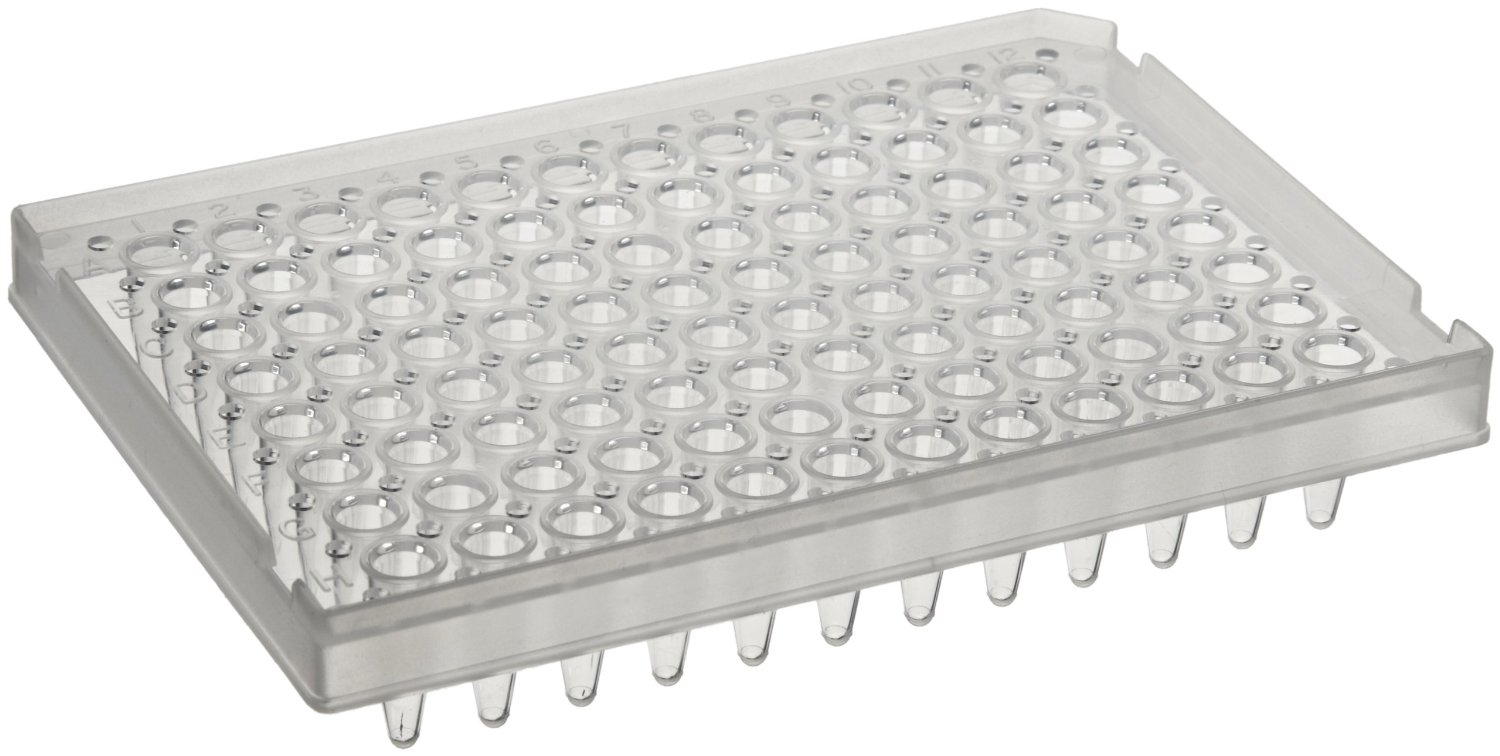
\includegraphics[width=0.8\textwidth]{96plate.png}
  \caption{A 96-well PCR plate.}
  \label{fig:96_well_plate}
\end{figure}

Upon receipt, some samples require human intervention to prepare them for sequencing. For instance, samples with uneven DNA concentrations must be normalized to ensure consistent sequencing quality. Additionally, samples that do not include a primer must have the appropriate primer added by laboratory staff. These steps are critical to ensure the accuracy and reliability of the sequencing results.

Once prepared, these plates are then loaded into the ABI3730xl DNA sequencer, which includes DNA denaturation, primer annealing, extension with fluorescently labeled dideoxynucleotides, and capillary electrophoresis. The ABI3730xl sequencer then generates raw data files containing fluorescence intensity readings, which are subsequently processed to produce DNA sequence alignments.


\subsection{The ABI3730xl DNA Sequencer}
The ABI3730xl DNA sequencer is a high-throughput instrument widely used in genomics for Sanger sequencing. It automates the electrophoresis and fluorescence detection steps, corresponding to steps 3 and 4 of the Sanger sequencing process (Figure \ref{fig:sanger_steps}), allowing for the simultaneous processing of 96-well plates in a single run \cite{smith_capillary_sequencing,abi3730xl_overview}. By leveraging this technology, laboratories can achieve precise and efficient DNA sequencing. 
\begin{figure}[h]
\centering
\includegraphics[width=0.7\textwidth]{abi_3730xl_closed.png}
\caption{A closed ABI3730xl capillary electrophoresis DNA analyzer.}
\label{fig:abi_3730xl_closed}
\end{figure}

\begin{figure}[h]
\centering
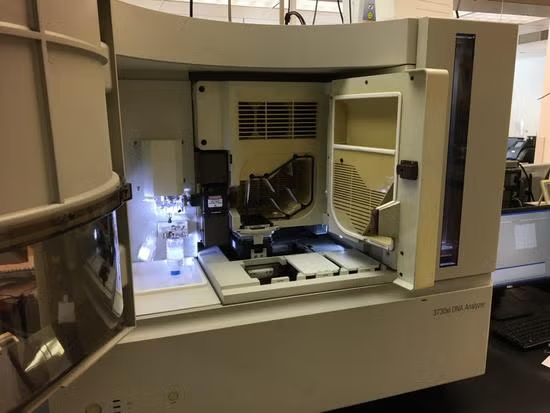
\includegraphics[width=0.7\textwidth]{abi_3730xl_opened.png}
\caption{An opened ABI3730xl capillary electrophoresis DNA analyzer.}
\label{fig:abi_3730xl_opened}
\end{figure}

\section{Data Structure and Analysis}
\label{sec:data_analysis }

The efficiency of any artificial intelligence model is heavily dependent on the quality and structure of the data used for training. In this work, the data originates from customer samples sequenced using the ABI3730xl sequencer. The sequencer outputs a variety of files, including raw fluorescence data, processed sequence alignments, and quality metrics.

Each 96-well plate generates a significant volume of data, with millions of files produced over time. These files are structured hierarchically, with each plate containing subdirectories for individual wells. The data includes:
\begin{itemize}
\item \textbf{Raw fluorescence traces}: These files contain the intensity readings for each of the four fluorescent dyes (A, T, C, G) used in Sanger sequencing.
\item \textbf{Processed sequence files}: These files contain the DNA sequences derived from the fluorescence traces, along with quality scores.
\item \textbf{Metrics and logs}: These files provide information on sequencing quality, including signal strength, noise levels, and potential errors.
\end{itemize}


% section document_structure (end)

